\documentclass[11pt]{article}
\usepackage[utf8]{inputenc}
\usepackage{geometry}
\usepackage{hyperref}
\usepackage{enumitem}
\usepackage{tikz}
\usepackage{booktabs}
\geometry{a4paper, margin=2.5cm}

\title{DICOM Conformance Statement \\ Web DICOM Viewer}
\author{Zargantana / Web DICOM Viewer}
\date{\today}

\begin{document}

\maketitle

\section*{1. Introduction}

This document is the DICOM Conformance Statement for the \textbf{Web DICOM Viewer}. This software component is designed for displaying DICOM images directly in a web browser. It supports uploading image files through a browser interface, visualizing them frame by frame with interactive navigation and rendering options.

\section*{2. Implementation Model}

\subsection*{2.1 Application Data Flow}

\begin{center}
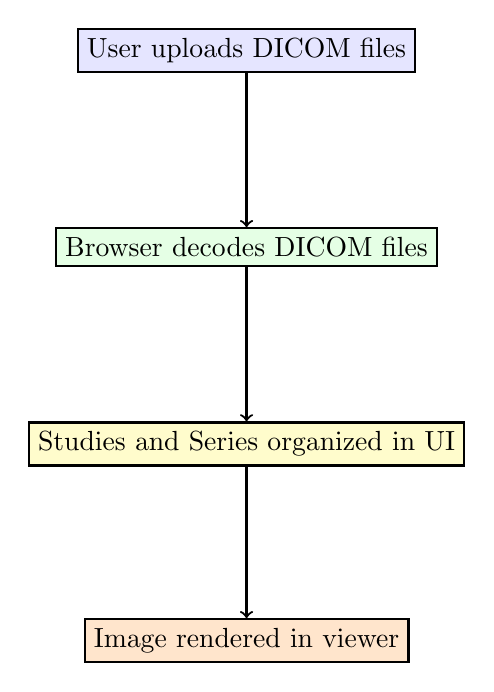
\begin{tikzpicture}[node distance=2.5cm, auto, thick]
  \node[draw, rectangle, fill=blue!10] (upload) {User uploads DICOM files};
  \node[draw, rectangle, below of=upload, fill=green!10] (decode) {Browser decodes DICOM files};
  \node[draw, rectangle, below of=decode, fill=yellow!20] (organize) {Studies and Series organized in UI};
  \node[draw, rectangle, below of=organize, fill=orange!20] (display) {Image rendered in viewer};

  \draw[->] (upload) -- (decode);
  \draw[->] (decode) -- (organize);
  \draw[->] (organize) -- (display);
\end{tikzpicture}
\end{center}

\subsection*{2.2 Functional Definition}
The Web DICOM Viewer is a \textbf{VIEWER} application that does not establish network communication via DICOM protocol (no SCU/SCP roles). It operates solely on files provided through user upload.

\section*{3. AE Specifications}

\subsection*{3.1 Web DICOM Viewer AE}

\begin{itemize}
  \item \textbf{SOP Classes Supported:}
  \begin{itemize}
    \item All storage SOP classes containing image data (e.g., CT, MR, XA, US, NM, CR, OT).
  \end{itemize}
  
  \item \textbf{Supported Transfer Syntaxes:}
  \begin{itemize}
    \item Explicit VR Little Endian (1.2.840.10008.1.2.1)
    \item Implicit VR Little Endian (1.2.840.10008.1.2)
    \item JPEG Baseline (Process 1) (1.2.840.10008.1.2.4.50)
    \item JPEG Lossless (1.2.840.10008.1.2.4.70)
    \item JPEG-LS Lossless (1.2.840.10008.1.2.4.80)
    \item JPEG 2000 Lossless (1.2.840.10008.1.2.4.90)
    \item RLE Lossless (1.2.840.10008.1.2.5)
  \end{itemize}
  
  \item \textbf{Image Display Capabilities:}
  \begin{itemize}
    \item Only the first defined window level (Window Center / Window Width) is used for rendering.
    \item Support for grayscale and color images as provided in the DICOM file.
  \end{itemize}
  
\end{itemize}

\subsection*{3.2 Supported Modalities}

\begin{center}
\begin{tabular}{ll}
\toprule
\textbf{Modality Code} & \textbf{Description} \\
\midrule
CR & Computed Radiography \\
US & Ultrasound \\
XA & X-Ray Angiography \\
NM & Nuclear Medicine (e.g., gammagraphy) \\
OT & Other (Generic / Non-standard) \\
DX & Digital Radiography \\
CT & Computed Tomography (if uploaded) \\
MR & Magnetic Resonance (if uploaded) \\
\bottomrule
\end{tabular}
\end{center}

\section*{4. Networking}

\textbf{Note:} This application does not support DICOM network communication (no DICOM Upper Layer Protocol, DICOMweb, or DIMSE services).

\section*{5. Browser Interface and User Interaction}

\begin{itemize}
  \item Users upload DICOM files via an HTML file input element.
  \item The system displays a list of studies and associated series.
  \item Users can select a study and navigate through its images.
  \item Two display modes:
    \begin{itemize}
      \item For studies with modality OT or more than 50 images: scroll navigation via mouse wheel.
      \item For other studies: a series list view with selection and optional cine loop playback.
    \end{itemize}
\end{itemize}

\section*{6. Limitations}

\begin{itemize}
  \item Only the first window level is supported.
  \item No support for DICOM C-FIND, C-MOVE, or other DICOM services.
  \item No integration with PACS or DICOMweb servers.
  \item Only file-based workflows supported.
\end{itemize}

\section*{7. Security}

The viewer operates entirely on the client side, without uploading data to a remote server. Security and confidentiality of patient data depend on user handling and browser environment.

\section*{8. IHE Integration Statement}

This viewer does not currently support IHE Integration Profiles such as RAD-68 or XDS-I.b.

\section*{9. Support and Contact Information}

Web DICOM Viewer \\
Website: \texttt{https://visordicom.es} \\
Email: \texttt{zargantana.reader@gmail.com}

\end{document}